\documentclass[12pt, a4paper]{article}
\usepackage[utf8]{inputenc}
\usepackage[english,russian]{babel}
\usepackage[T1, T2A]{fontenc}
\usepackage{graphicx}
\usepackage{epstopdf}
\usepackage{caption}
\usepackage{threeparttable}
\usepackage[margin=14pt,font=small,labelsep=endash]{caption}
\captionsetup[figure]{labelformat=simple, labelsep = endash, name = Рисунок}
\captionsetup[table]{name = Таблица, labelsep = endash, justification=raggedright, singlelinecheck=false}
\usepackage{float}
\usepackage{geometry} %способ ручной установки полей
\geometry{top=2cm} %поле сверху
\geometry{bottom=2cm} %поле снизу
\geometry{left=2cm} %поле справа
\geometry{right=2cm} %поле слева
\usepackage{amsmath}
\newcommand\tline[2]{$\underset{\text{#1}}{\text{\underline{\hspace{#2}}}}$}
\newcommand\nameLine[3]{$\underset{\text{#1}}{\text{\underline{\text{#2}\hspace{#3}}}}$}

%opening
\title{}
\author{}

\begin{document}
\begin{titlepage}
		\centering
		{\fontsize{12pt}{5cm}\selectfont \bfseries Министерство образования и науки Российской Федерации} \\ \vspace{0.5cm}
		{\fontsize{7pt}{5cm}\selectfont ФЕДЕРАЛЬНОЕ ГОСУДАРСТВЕННОЕ АВТОНОМНОЕ ОБРАЗОВАТЕЛЬНОЕ УЧРЕЖДЕНИЕ ВЫСШЕГО ПРОФЕССИОНАЛЬНОГО ОБРАЗОВАНИЯ} \\ 
		\vspace{1cm}
		{\fontsize{12pt}{5cm}\selectfont \bfseries САНКТ-ПЕТЕРБУРГСКИЙ УНИВЕРСИТЕТ ИНФОРМАЦИОННЫХ ТЕХНОЛОГИЙ, МЕХАНИКИ И ОПТИКИ} \\ \vspace{1.5cm}

		{\fontsize{14pt}{5cm}\selectfont Кафедра \hspace{1cm} \underline{Систем Управления и Информатики}  \hspace{1cm} Группа \underline{Р3340}} \\ 
		\vspace{2cm}

		{\fontsize{20pt}{5cm}\selectfont \bfseries Лабораторная работа №12} \\
		{\fontsize{20pt}{5cm}\selectfont \bfseries Анализ линейных непрерывных систем с использованием прикладного пакета Matlab Control System Toolbox} \\
		{\fontsize{14pt}{5cm}\selectfont Вариант - 9} \\
		\vspace{1.5cm}

		\flushleft

		{Выполнила \hspace{1,7cm} \nameLine{(фамилия, и.о.)}{Сорокина Т. В.}{6.3cm} (подпись)} \\
		\vspace{2cm}

		{Проверил \hspace{2cm} \tline{(фамилия, и.о.)}{9cm} (подпись)} \\
		\vspace{5cm}

		"\underline{\hspace{0.7cm}}"\hspace{0.2cm}\underline{\hspace{2cm}}\hspace{0.2cm}20\underline{\hspace{0.7cm}}г. \hspace{2cm} Санкт-Петербург, \hspace{2cm} 20\underline{\hspace{0.7cm}}г. \\ \vspace{1cm}

		Работа выполнена с оценкой \hspace{1cm} \underline{\hspace{8cm}} \\ 
		\vspace{1cm}
		Дата защиты "\underline{\hspace{0.7cm}}"\hspace{0.2cm}\underline{\hspace{2cm}}\hspace{0.2cm}20\underline{\hspace{0.7cm}}г.

	\end{titlepage}
%\maketitle
%\begin{abstract}
%\end{abstract}

\paragraph {Цель работы:} исследование динамических и частотных характеристик, анализ структурных свойств и устойчивости линейных непрерывных систем, с помощью прикладного пакета Matlab Control System Toolbox. \\
\textbf{Исходные данные}
\par 
Исходная модель разомкнутой системы представляется в форме вход-выход и
описывается передаточной функцией вида:
\begin{equation} 
W(s) = \frac{b_1s+b_0}{s\cdot(a_2s^2+a_1s+a_0)}.
\end{equation}

Значения коэффициентов $a_0, a_1, a_2, b_0, b_1$ в числителе и знаменателе передаточной функции для выполнения лабораторной работы выбираются самостоятельно произвольно из условия $a_2\neq0, b_1\neq0$.\par 
Выбранные значения коэффициентов: $a_0=4, a_1=2, a_2=1, b_0=-3, b_1=6$.
Тогда передаточная функция будет выглядеть следующим образом:
\begin{equation} 
W(s) = \frac{6s-3}{s\cdot(s^2+2s+4)}.
\end{equation}

\newpage
\begin{center}
\section{Анализ исходной разомкнутой системы}
\end{center}

\par Найдём нули и полюса передаточной функции разомкнутой системы (используя функцию Рole-Zero map), результат представим в виде графика, который изображен на рисунке 1.
\parНули передаточной функции (корни числителя):
z=0.5.
\par Полюса передаточной функции (корни знаменателя):
$p_{1}=0$, $p_{2}=-1-i\sqrt{3}$, \\$p_{3}=-1+i\sqrt{3}$


\begin{figure}[H]
\centering
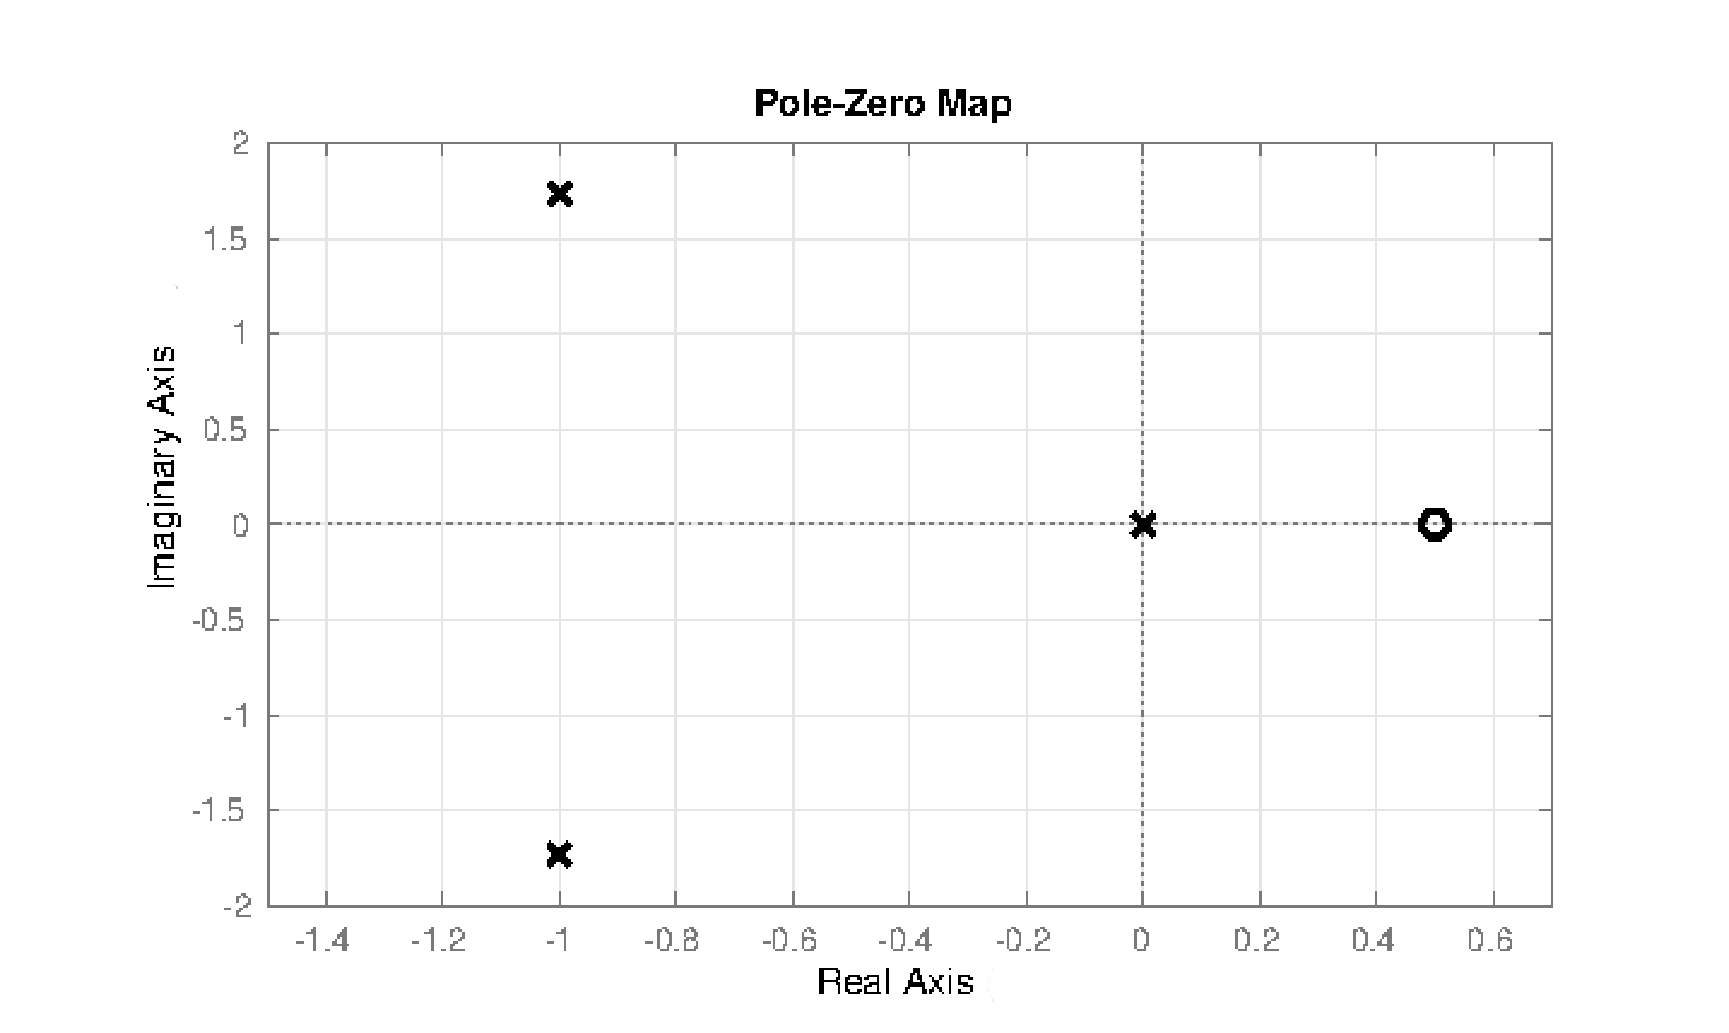
\includegraphics[width=0.8\textwidth]{1/im1.eps}
\caption{Нули и полюса разомкнутой системы}
\end{figure}
\par Система находится на нейтральной границе устойчивости, так как имеет нулевой полюс, но не имеет полюсов с положительной вещественной частью.
\par Воспользуемся функцией Bode для нахождения ЛАЧХ и ЛФЧХ. Графики ЛАЧХ и ЛФЧХ изображены на рисунке 2. 
\begin{figure}[H]
\centering
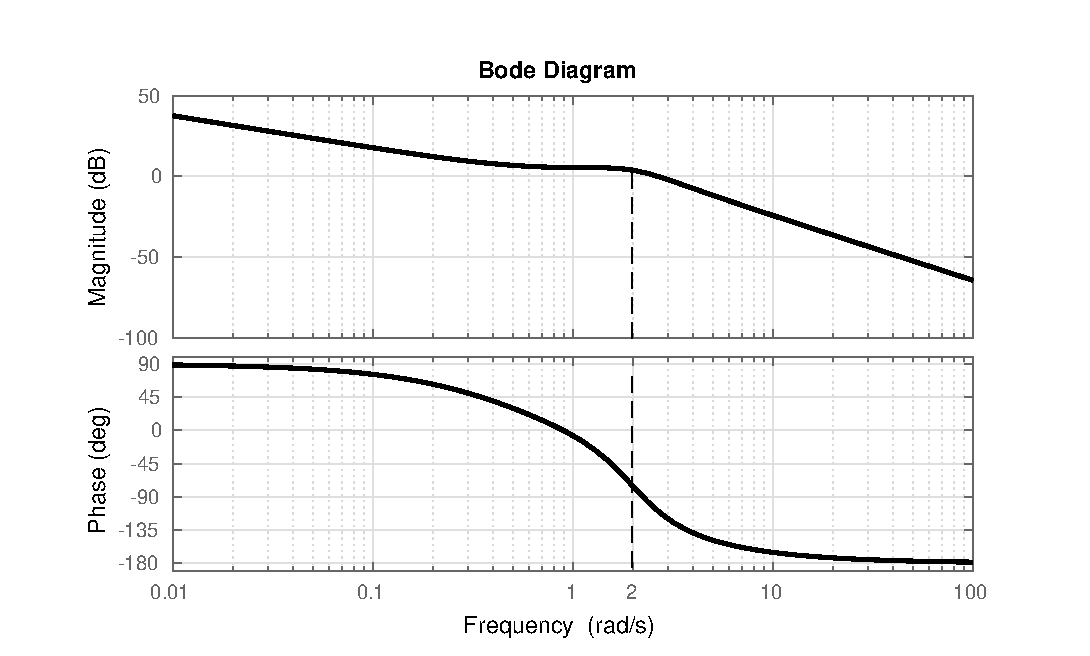
\includegraphics[width=0.8\textwidth]{1/bode2.eps}
\caption{Логарифмические характеристики разомкнутой системы}
\end{figure}
\par Используя функцию margin найдем запасы по амплитуде и частоте. Запас устойчивости системы по амплитуде - бесконечный, частота среза = 2 рад/с,
запас устойчивости по фазе равен 70,95 градусов.
\par Используя функцию Nyquist plot построим АФЧХ исследуемой системы. АФЧХ исследуемой системы приведена на рисунке 3.
\begin{figure}[H]
\centering
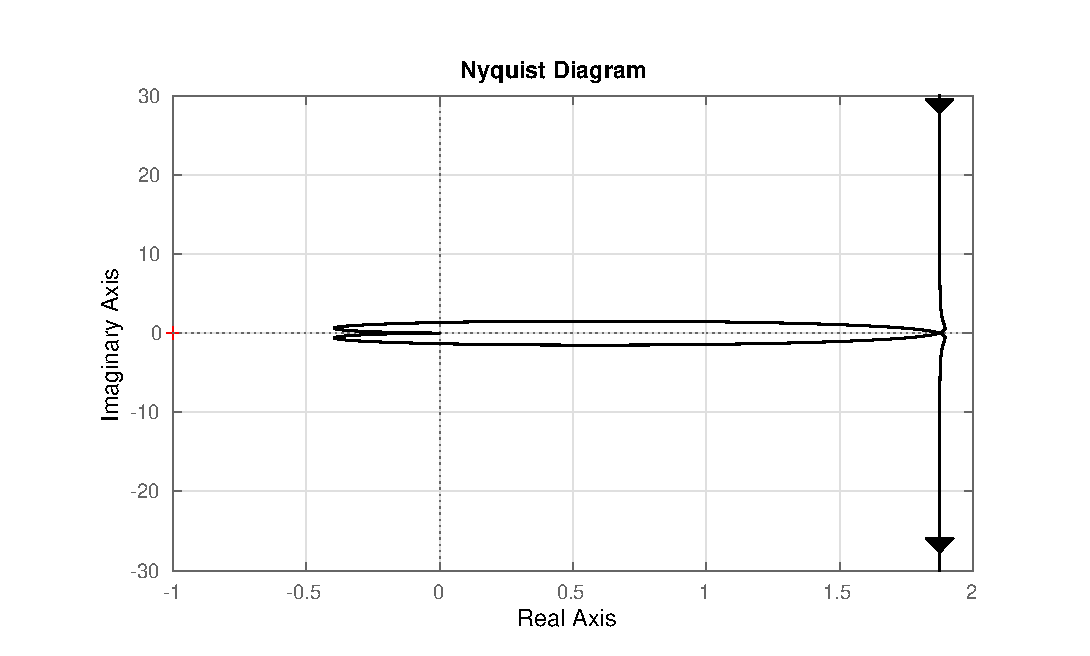
\includegraphics[width=0.8\textwidth]{1/nyq1.eps}
\caption{АФЧХ разомкнутой системы}
\end{figure}
\par Система является устойчивой по критерию Найквиста, так как АФЧХ системы не охватывает точку (-1;0).


\newpage
\begin{center}
\section{Анализ замкнутой системы }
\end{center} \par

Передаточная функция системы с  отрицательной обратной связью в нашем случае будет иметь вид:
\begin{equation}
\Phi(s) = \frac{\displaystyle{\frac{6s - 3}{s^3 + 2s^2 + 4s}}}{1 + \displaystyle{\frac{6s - 3}{s^3 + 2s^2 + 4s}}\cdot K} = \frac{6s - 3}{s^3 + 2s^2 + (4 + 6K)s - 3K}
\end{equation}\par
\par Проанализируем влияние коэффициентов отрицательной обратной связи на расположение полюсов передаточной функции.Для этого будем использовать
функцию rlocus. На рисунке 4 приведена зависимость расположения полюсов замкнутой системы от коэффициента обратной связи.
\begin{figure}[H]
\centering
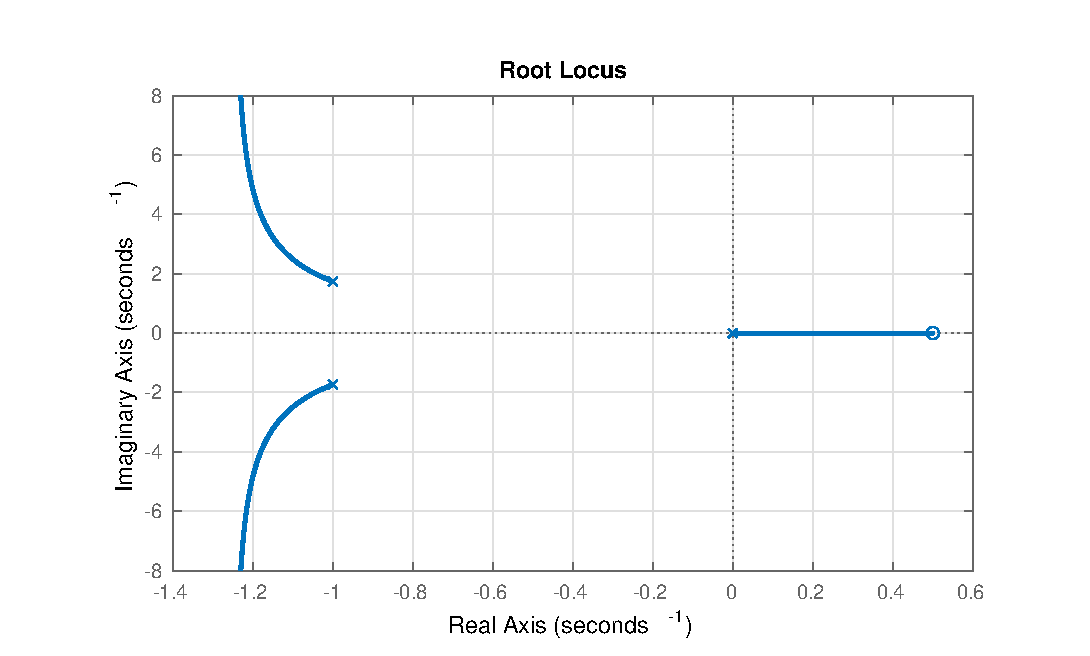
\includegraphics[width=0.8\textwidth]{1/rlocus.eps}
\caption{Зависимость расположения полюсов замкнутой системы от коэффициента обратной связи}
\end{figure}

Для выбора коэффициента К воспользуемся корневым критерием устойчивости и составим матрицу Гурвица:
\[
\begin{vmatrix}
2 & -3K & 0\\
1 & 4+6K & 0\\
0 & 2 & -3K
\end{vmatrix}
\]
\par Отсюда видно, что при К=0 система будет находится на нейтральной границе устойчивости. Система будет находится на колебательной границе 
устойчивости при К=-0,53. И система будет устойчива при К в диапозоне от -0,53 до 0.
\par Выберем коэффициент К=-0,4. Тогда система примет вид:
\begin{equation}
\Phi(s) = \frac{6s - 3}{s^3 + 2s^2 + 1,6s + 1,2}
\end{equation}
\par Найдем значения нулей и полюсов для замкнутой системы. Графическое изображение нулей и полюсов замкнутой системы представлено на рисунке 5.
\\z=0.5, $p_{1}=-1.467$ 
\\$p_{2}=-0.266-0.864i$, $p_{3}=-0.266+0.864i$.

\begin{figure}[H]
\centering
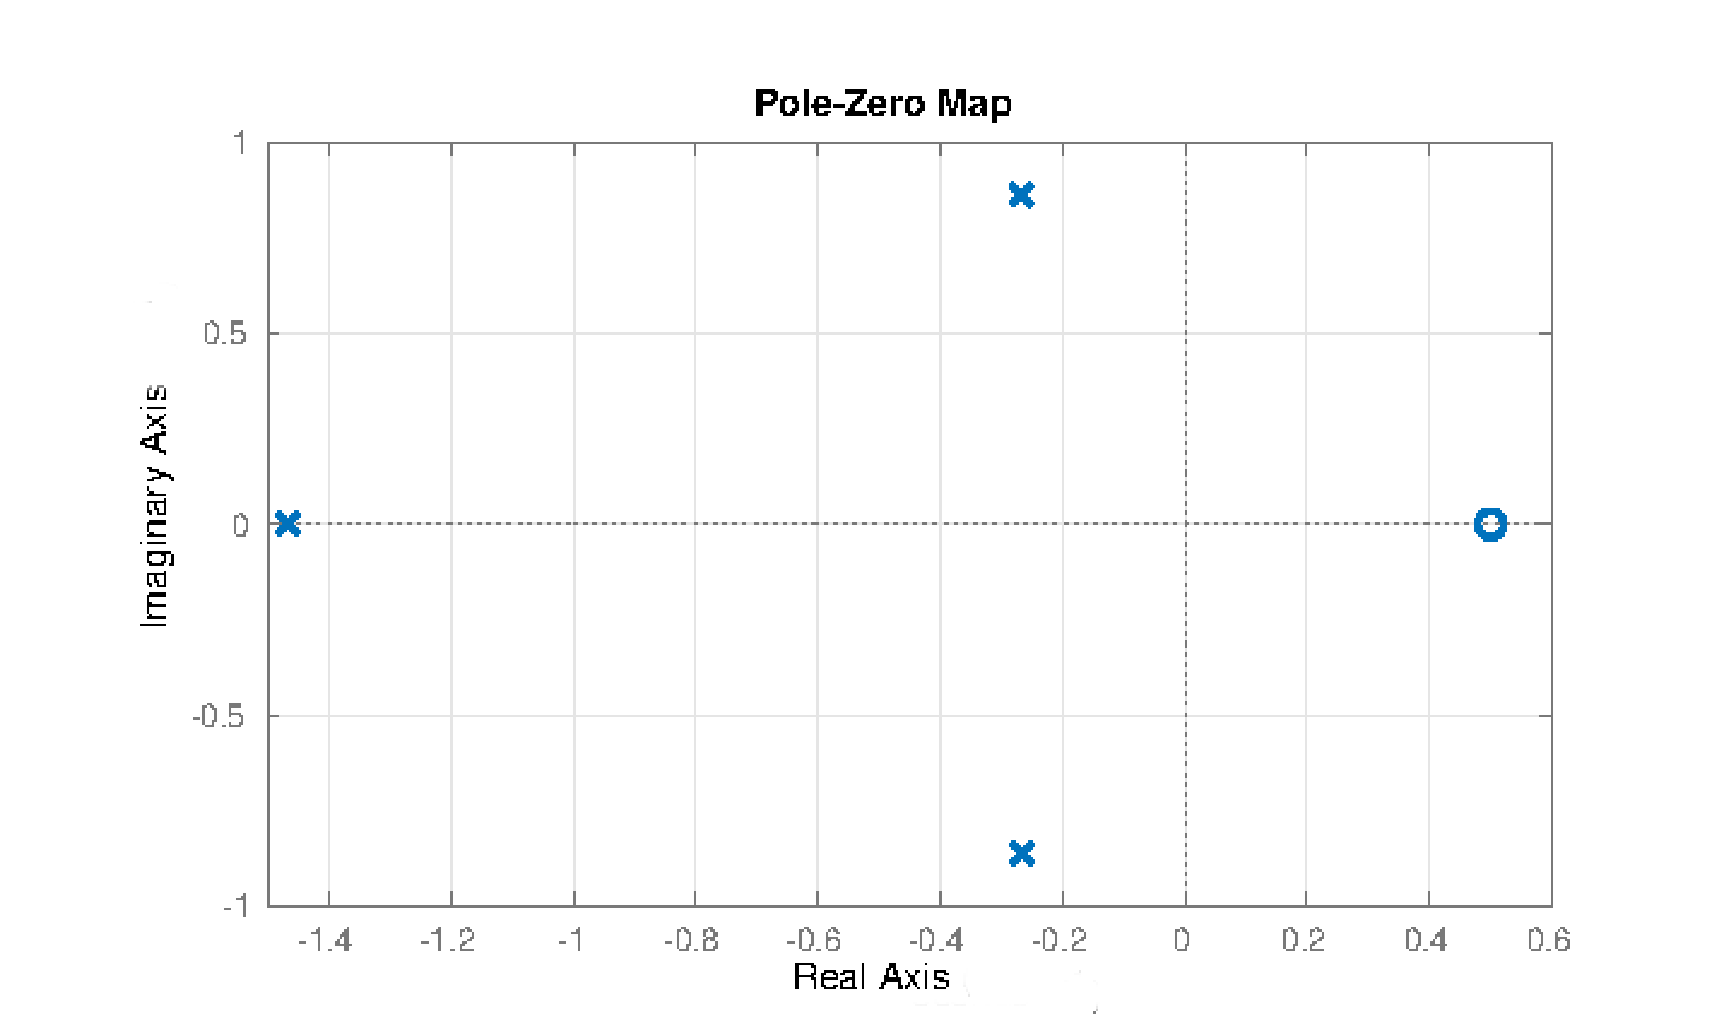
\includegraphics[width=0.8\textwidth]{1/im3.eps}
\caption{Нули и полюса замкнутой системы}
\end{figure}
\par Система является устойчивой, т.к. не имеет корней с неотрицательной вещественной частью. Степень устойчивости в данном случае будет
вычисляться как:
\begin{equation}
    |Re (p_2)| = |Re(p_3)| = 0,266.
\end{equation}

\par Выполним построение графиков переходной и весовой функции замкнутой системы, применив функции: step, impulse.
Данные графики приведены на рисунках 6 и 7. 
\begin{figure}[H]
\centering
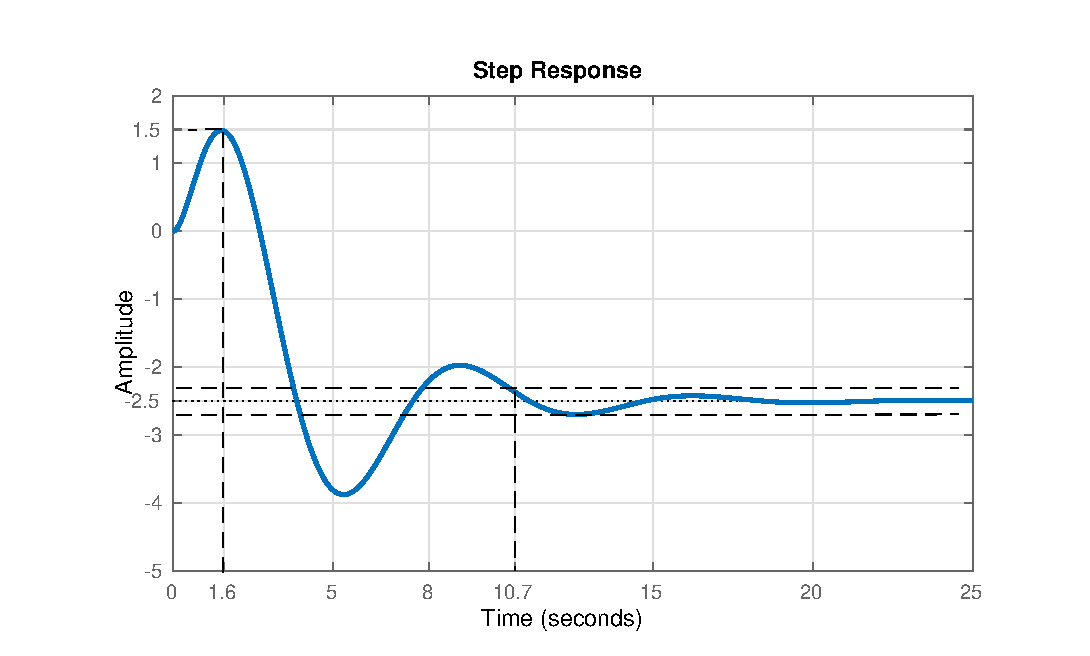
\includegraphics[width=0.8\textwidth]{1/step.eps}
\caption{График переходной функции замкнутой системы}
\end{figure}

\begin{figure}[H]
\centering
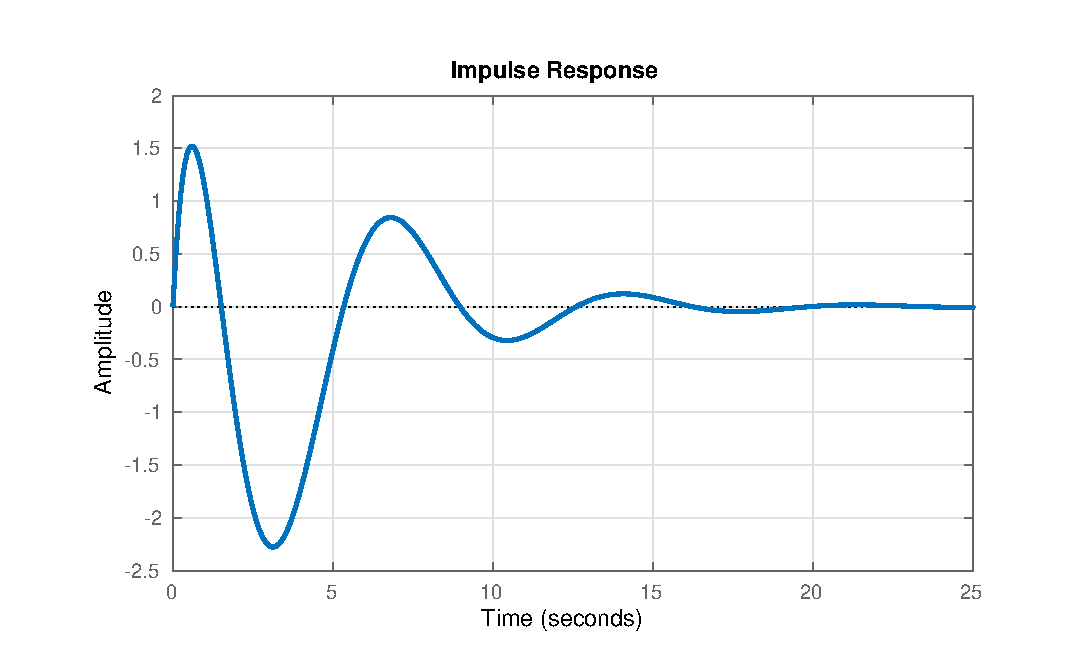
\includegraphics[width=0.8\textwidth]{1/impulse.eps}
\caption{График весовой функции замкнутой системы}
\end{figure}
 \par Определим по графику время переходного процесса: $t_\text{п}$=10,7 с. 
 \par Значение перерегулирования: $\sigma=\displaystyle{\frac{1,5+2,5}{-2,5}\cdot100\%=160\%}$
 \par Затухание равно 0.
 \par Перейдем к представлению замкнутой системе в форме Вход-Состояние-Выход. С помощью функции [A,B,C,D] = tf2ss(b,a), получим матрицы:
 
\begin{equation*}
A =\begin{bmatrix}
    -2      &   -1,6   &   -1,2 \\
    1       &   0   &	0 \\
    0    & 1  &   0
\end{bmatrix}
\end{equation*}
\begin{equation*}
B =\begin{bmatrix}
    1 \\
	0  \\
	0
\end{bmatrix}
\end{equation*}
\begin{equation*}
C =\begin{bmatrix}
    0 & 6  & -3 \\
\end{bmatrix}
\end{equation*}

\par Найдем матрицы управляемости и наблюдаемости, используя команды: ctrb(A,B) и obsv(A,C).
\begin{equation*}
U_y =\begin{bmatrix}
    1   &   -2   &   2,4 \\
    0   &   1   &	-2 \\
    0   &   0  &   1
\end{bmatrix}
\end{equation*}
\begin{equation*}
U_n =\begin{bmatrix}
    0    &   6       &   -3 \\
    6       &   -3      &	0 \\
    -15   &   9,6   &   -7,2
\end{bmatrix}
\end{equation*}\par
Так как ранги матриц $U_{y}$ и $U_n$ равны порядку системы (ранг матриц = 3), то можно заключить, что система является полностью
управляемой и наблюдаемой.
\newpage
\begin{center}
\section*{Вывод} 
\end{center}
 \par  В данной лабораторной работе был использован прикладной пакет Matlab Control System Toolbox. С его помощью было проведено исследование 
 динамических и частотных характеристик, анализ структурных свойств и устойчивости линейных непрерывных систем.
 \par Используя функцию pzmap были найдены полюса и нули передаточной функции как разомкнутой системы, так и  замкнутой.
 \par При использовании функции Bode были построены ЛАЧХ и ЛФЧХ, по которым были найдены: частота среза и запасы устойчивости по амплитуде и фазе.
 \par Так же при выполнении лабораторной работы была применена функция Nyquist plot,которая строит АФЧХ исследуемой системы. 
 \par С помощью функций step и impulse были получены графики переходных функций, по которым были найдены: время переходного процесса,
 значение перерегулирования и затухание замкнутой системы.
 \par С помощью функции [A,B,C,D]=tf2ss(b,a) получили матрицы ВСВ. Используя команды: ctrb (A,B) и obsv (A,C) 
 получили матрицы управляемости и наблюдаемости.
 \end{document}

